\documentclass{standalone}
\usepackage{amsmath}
\usepackage[dvipsnames]{xcolor}
\usepackage{tikz} 
\usetikzlibrary{arrows, decorations.markings,decorations.pathreplacing,angles,quotes}
\usepackage{microtype}
\usepackage{fourier}

%include other needed packages here   
\begin{document}

\begin{tikzpicture}
% include your tikz code here
    		\node[anchor=south west,inner sep=0] (Bild) at (0,0) {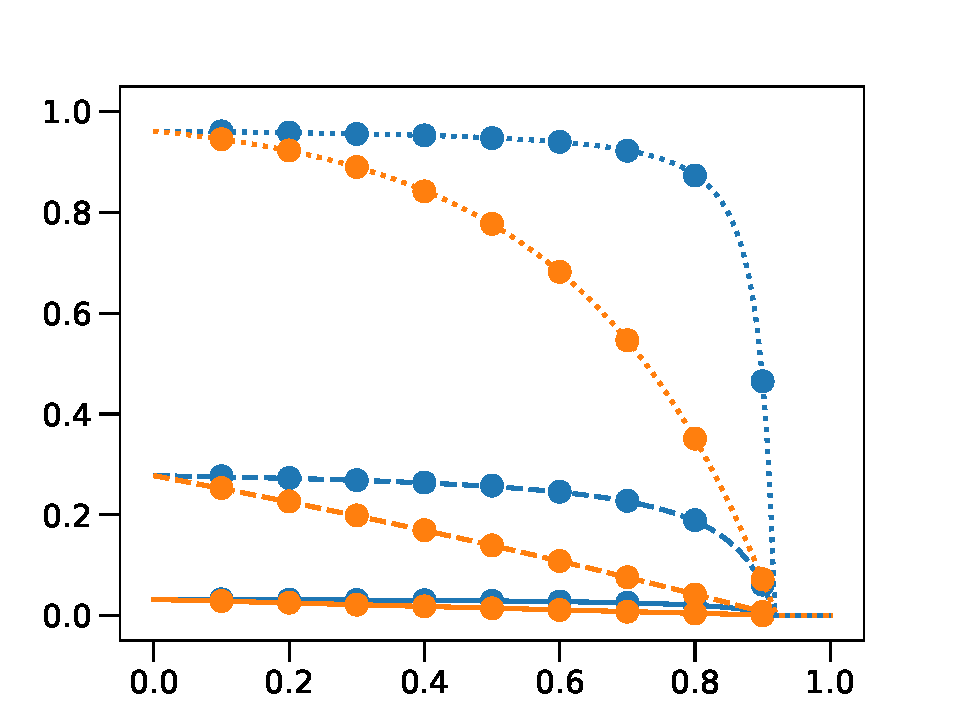
\includegraphics[scale=0.39]{figS6b_blank.pdf}};
   		\begin{scope}[x=(Bild.south east),y=(Bild.north west)]
        	\draw (0.55,-0.035) node {antiviral drug efficacy $\varepsilon_j$};
        	\draw (0.01,0.5) node [rotate=90] {establishment probability $\varphi$};
        	%\draw[blue,thick] (0.175,0.77) -- node[right=6pt] {\scriptsize \color{black} reducing burst size $B$} (0.225,0.77);
        	%\draw[orange,thick] (0.175,0.7) -- node[right=6pt] {\scriptsize \color{black} reducing infectivity $\beta$} (0.225,0.7);
        	%\draw[black,thick] (0.175,0.4) -- node[right=6pt] {\scriptsize \color{black} $V_0=1$} (0.225,0.4);
        	%\draw[black,thick,dashed] (0.175,0.33) -- node[right=6pt] {\scriptsize \color{black} $V_0 = 10$} (0.225,0.33);
        	%\draw[black,thick,dotted] (0.175,0.26) -- node[right=6pt] {\scriptsize \color{black} $V_0 = 100$} (0.225,0.26);
    		\end{scope}
\end{tikzpicture}

\end{document}